\section{Networking Theory and Protocols}
In a multi-network system consisting of multiple edges with different transmission mediums and nodes with different services running on it, communication between different entities in the network happens on different levels. Communication on the lowest levels is characterized by simple byte transmissions over a given medium between two or more directly connected nodes of the network while on the highest levels it is characterized by complex dialogs of data exchange between different applications running on different nodes in different networks. Every new layer in this hierarchy adds a level of abstraction on top of all layers below to handle evermore complex kinds of communication between entities in the network.

The following section will give a short introduction into the widely used OSI model of this layering scheme. The subsequent sections will then explore the various technologies used in this project, which implement some of those layers.

\subsection{Open Systems Interconnection (OSI) Model}
The Open Systems Interconnection (OSI) model is the most widely used model of the networking communication layers. It defines seven distinct layers of increasing abstraction, where each layer handles the implementation of a special kind of communication system by utilizing the layers below it. The seven layers of the OSI model from bottom to top are:
\begin{enumerate}
  \item \texttt{Physical Layer:} Implements the raw transmission of bits over a medium shared by two or more link partners. It only handles direct connections between those link partners over wired (copper cables, fiber cables, etc.) or wireless (radio signals) connection methods and ensures, that transmitted information reaches all link partners without loss of information.
  \item \texttt{Data Link Layer:} Implements the safe transmission of data over a medium shared by two or more link partners. Based on the physical layer it wraps transmissions in packets and assigns addresses and checksums to the transmitted data to ensure, that data is transmitted without undetectable errors to the intended recipient.
  \item \texttt{Network Layer:} Implements routing of packets through multiple networks. Different networks must be connected by routers. It uses special network addresses for routing. It uses the data link layer.
  \item \texttt{Transport Layer:} Implements communication between different applications or services on different entities in connected networks. It can handle connections and provides additional reliability methods and flow control. It uses the network layer.
  \item \texttt{Session Layer:} Implements communication in sessions between entities. It uses the transport layer.
  \item \texttt{Presentation Layer:} Implements data format conversions between the lower layers and the application layer.
  \item \texttt{Application Layer:} Represents the actual applications running on nodes in the network. Those applications can communicate with other applications on other nodes in the network by utilizing all other layers below.
\end{enumerate}
Although the OSI model gives a useful model for the network communication layers, in reality those layers are not strictly implemented separately, since optimizations between those layers often require them to be handled together.

\subsection{Fast Ethernet (IEEE 802.3u)}
Fast ethernet, standardized by IEEE as 802.3u, is a standard located in the IEEE 802.3 working group for wired ethernet (\cite{ieee:802.3}) which is itself located in the IEEE 802 family of standars for networks carrying variable-size packets (\cite{wikipedia.org:ieee_802}). Specifically, 802.3u establishes various standards for wired communication over a network in a transmission speed of 100 Mbit/s and twisted-pair or fiber cables as transmission medium. Fast ethernet over twisted-pair cables, which is the most common connection, is called 100BASE-TX and requires network cables of category Cat-5 or better.
The target of the 802.3u standard can be divided in two parts. The first one regarding the low level part of ethernet describes, how transmission of bits over the given medium is generally handled with no regard of the structure of the transmitted data and corresponds to the physical layer (layer 1) of the OSI model. The second one regarding the higher level part of ethernet describes, how data is being exchanged between two link partners and corresponds to the data link layer (layer 2) of the OSI model. Those two parts are generally implemented by different hardware, which are connected via the Media Independent Interface (MII), which is also part of 802.3u, or one of its improvements (RMII, GMII, etc.). The following sections will provide further information about the two parts and the connecting interface.

\subsubsection{Low Level Transmission of Bits}
This part corresponds to the OSI physical layer (layer 1).

Low level transmission encompasses all tasks to be performed to successfully transmit single bits over a given medium. These tasks can be divided into the following categories \cite{smsc:lan8720a}:
\begin{itemize}
  \item Encoding of outgoing and decoding of incoming data with a format suitable for transmission,
  \item Feature negotiation between link partners (transmission speed, half or full duplex mode, etc.),
  \item Recovery of incoming data from signals with phase and amplitude distortions due to disturbances while transmission.
\end{itemize}

Usually, the physical layer is implemented by a chip commonly called a "PHY", meaning it handles the tasks of the physical layer.

\subsubsection{Reduced Media Independent Interface}
The Media Independent Interface (MII) and all its advanced versions like the used Reduced Media Independent Interface (RMII) are an established standard interface for connecting the Media Access Control (MAC) to an ethernet PHY. The MAC is defined by this relationship. This ensures, that MACs need not to be modified, if another transmission medium is required to be used.

In this project, the RMII has been used, therefore only this version will be described here.

The signals defined in the specification for the RMII are listed in table \ref{table:rmii_signals}. REF\_CLK is the clock signal for data transmission and can be either a 50 MHz clock for 100 Mbit/s or a 5 MHz clock for 10 Mbit/s transmission speed. RXD is the data signal for incoming data. The PHY will set it, if it receives the next two bits of data. Data is valid, if CRS\_DV is asserted. If there has been an error while receiving the current two bits, RX\_ER is asserted. Outgoing data must be set at TXD two bits per clock cycle. The PHY will send those two bits out if TX\_EN is asserted. Transmissions of data of more than two bits are handled by consecutively handling all byte pairs of the message. \textbf{Important! TXD[0] is the first transmitted bit, RXD[0] is the first received bit.}

\begin{table}[]
  \centering
  \begin{tabular}{|c|c|c|c|}
    \hline
    \textbf{Signal name} & \textbf{\begin{tabular}[c]{@{}c@{}}Direction\\ (PHY)\end{tabular}} & \textbf{\begin{tabular}[c]{@{}c@{}}Direction\\ (MAC)\end{tabular}} & \textbf{Use} \\ \hline
    REF\_CLK & Input & \begin{tabular}[c]{@{}c@{}}Input or\\ Output\end{tabular} & \begin{tabular}[c]{@{}c@{}}Synchronous clock reference\\ for receive, transmit\\ and control interface\end{tabular} \\ \hline
    CRS\_DV & Output & Input & Carrier Sense/Receive Data Valid \\ \hline
    RXD{[}1:0{]} & Output & Input & Receive data \\ \hline
    TX\_EN & Input & Output & Transmit enable \\ \hline
    TXD{[}1:0{]} & Input & Output & Transmit data \\ \hline
    RX\_ER & Output & \begin{tabular}[c]{@{}c@{}}Input\\ (not required)\end{tabular} & Receive Error \\ \hline
  \end{tabular}
  \caption[Signals of the RMII specification]{Signals of the RMII specification. Taken from the official specification (\cite{rmii:spec}).}
  \label{table:rmii_signals}
\end{table}

\subsubsection{Higher Level Transmission of Data}
This part corresponds to the OSI data link layer (layer 2).

It defines that data is transmitted in packets and how those packets are shaped and handled upon receiving.

MAC packets are the lowest level packets. The structure of a MAC packet is shown in figure~\ref{figure:mac_packet}. The fields of a MAC packet are:
\begin{itemize}
  \item \textbf{Preamble:} Sequence 10101010 10101010 10101010 10101010 10101010 10101010 10101010. \textbf{This sequence is transmitted from left to right.}
  \item \textbf{Start of Frame Delimiter (SFD):} Sequence 10101011. \textbf{This sequence is transmitted from left to right.}
  \item \textbf{Destination Address:} MAC address of packet recipient. \textbf{This address is transmitted least significant bit first octet-wise.}
  \item \textbf{Source Address:} MAC address of packet sender. \textbf{This address is transmitted least significant bit first octet-wise.}
  \item \textbf{Length / Type:} Number of octets in the mac client data (if value smaller or equal to 1500) or protocol used in mac client data (if value bigger or equal to 1536). For an embedded IP packet, the type value would be set as 0x0800. \textbf{This value is transmitted least significant bit first octet-wise.}
  \item \textbf{MAC Client Data:} Packet payload. Here are second level packets embedded. Must be between 46 and 1500 octets. If it is smaller than 46 octets, padding octets are added until the size is 46. \textbf{This value is transmitted least significant bit first octet-wise.}
  \item \textbf{Padding (PAD):} Padding octets included to ensure minimal packet length.
  \item \textbf{Frame Check Sequence (FCS):} CRC32 checksum of the packet. Calculated over the packet from MAC Destination Address through the payload. Calculation is described in section \ref{section:fcs}. \textbf{This value is transmitted most significant bit first, where the most significant bit is the coefficient belonging to the term \(x^{31}\) and the least significant bit is the coefficient belonging to the term \(x^0\).}
\end{itemize}

Between packets, there must be a transmission pause of 12 octets.

\begin{figure}[h]
  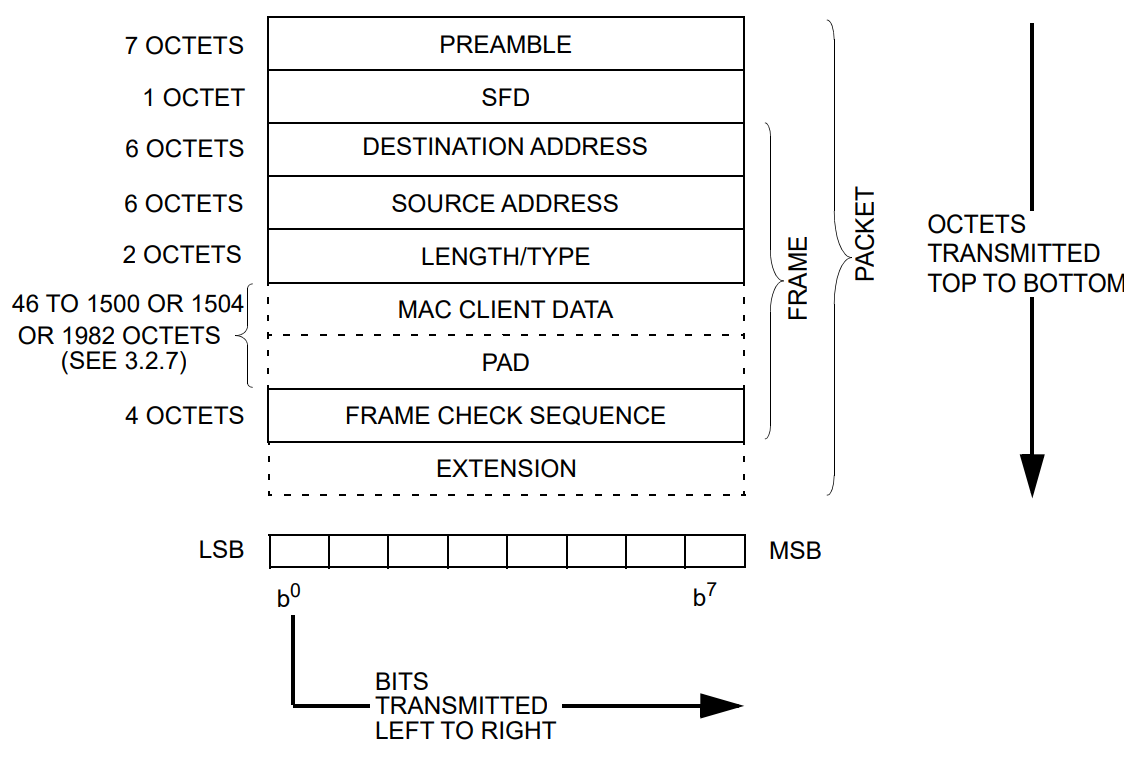
\includegraphics[width=\textwidth]{assets/mac_frame.png}
  \caption[Structure of an ethernet packet]{Structure of an ethernet packet. Field names are transmitted consecutively from top to bottom. TX\_EN is asserted while transmitting all fields except IPG.}
  \source{IEEE Standard for Ethernet~\cite{ieee:802.3}, page 119}
  \label{figure:mac_packet}
\end{figure}

\subsection{Internet Protocol Version 4 (RFC 791)}
This protocol corresponds to the OSI network layer (layer 3).

The IP protocol packet is used for routing packets over ethernet from one device to another over multiple networks utilizing 32 bit addresses. The structure of an IP packet is shown in table \ref{table:IP_packet}. The fields of an IP packet are:

\newcolumntype{C}[1]{>{\centering\let\newline\\\arraybackslash\hspace{0pt}}m{#1}}

\begin{sidewaystable}
  \centering
  \begin{tabular}{|c*{32}{|@{}C{5mm}@{}}|}
  \hline
  \footnotesize{\textbf{Offset}} & \footnotesize{\textbf{0}} & \footnotesize{\textbf{1}} & \footnotesize{\textbf{2}} & \footnotesize{\textbf{3}} & \footnotesize{\textbf{4}} & \footnotesize{\textbf{5}} & \footnotesize{\textbf{6}} & \footnotesize{\textbf{7}} & \footnotesize{\textbf{8}} & \footnotesize{\textbf{9}} & \footnotesize{\textbf{10}} & \footnotesize{\textbf{11}} & \footnotesize{\textbf{12}} & \footnotesize{\textbf{13}} & \footnotesize{\textbf{14}} & \footnotesize{\textbf{15}} & \footnotesize{\textbf{16}} & \footnotesize{\textbf{17}} & \footnotesize{\textbf{18}} & \footnotesize{\textbf{19}} & \footnotesize{\textbf{20}} & \footnotesize{\textbf{21}} & \footnotesize{\textbf{22}} & \footnotesize{\textbf{23}} & \footnotesize{\textbf{24}} & \footnotesize{\textbf{25}} & \footnotesize{\textbf{26}} & \footnotesize{\textbf{27}} & \footnotesize{\textbf{28}} & \footnotesize{\textbf{29}} & \footnotesize{\textbf{30}} & \footnotesize{\textbf{31}} \\ 
  \hline
  0 & \multicolumn{4}{c|}{Version} & \multicolumn{4}{c|}{IHL} & \multicolumn{6}{c|}{DSCP} & \multicolumn{2}{@{}c@{}|}{ECN} & \multicolumn{16}{c|}{Total Length} \\ 
  \hline
  32 & \multicolumn{16}{c|}{Identification} & \multicolumn{3}{c|}{Flags} & \multicolumn{13}{c|}{Fragment Offset} \\ 
  \hline
  64 & \multicolumn{8}{c|}{Time to Live} & \multicolumn{8}{c|}{Protocol} & \multicolumn{16}{c|}{Header Checksum (optional)} \\ 
  \hline
  96 & \multicolumn{32}{c|}{Source IP Address} \\ 
  \hline
  128 & \multicolumn{32}{c|}{Destination IP Address} \\ 
  \hline
  160 & \multicolumn{32}{c|}{\multirow{3}{*}{Options (optional)}} \\ 
  \cline{1-1}
  ... & \multicolumn{32}{c|}{} \\ 
  \cline{1-1}
  448 & \multicolumn{32}{c|}{} \\
  \hline
  \end{tabular}
  \caption[Structure of an IP packet]{Structure of an IP packet. The first row and the leftmost column indicate the index of the bit.}
  \label{table:IP_packet}
\end{sidewaystable}

\begin{itemize}
  \item \textbf{Version:} The version of the IP protocol. Always 0x4 for IPv4.
  \item \textbf{IP Header Length (IHL):} Defines the length of the header in 32-bit words. A value of 0x5 means the normal header size of 20 bytes / 160 bits is used. Smaller values are not allowed. Bigger values enable optional options at the end of the header, which can be used for custom applications.
  \item \textbf{Differentiated Services Code Point (DSCP):} Very special options not needed for the vast majority of all IP applications.
  \item \textbf{Explicit Congestion Notification (ECN):} Same as DSCP.
  \item \textbf{Total Length:} Total length in bytes of an IP packet. It does not include inserted paddings of the ethernet packet for too small payloads.
  \item \textbf{Identification:} Unique identifier for packet. Used to assemble different fragments of the same packets.
  \item \textbf{Flag 1 / Reserved:} Always 0.
  \item \textbf{Flag 2 / Don't Fragment (DF):} If set, packet must not be fragmented.
  \item \textbf{Flag 3 / More Fragments (MF):} If set, there are more fragments of the packet. Not set on the last fragment.
  \item \textbf{Fragment Offset:} Offset to start of packet of the current fragment.
  \item \textbf{Time to Live (TTL):} Number of times the packet is passed along until it is dropped. This ensures, packets will not congest networks if stuck in a looped path.
  \item \textbf{Protocol:} Defines the used protocol of the packet within the payload. E.g. for UDP this value is 0x11.
  \item \textbf{Header Checksum:} This a simple checksum of the header values (excluding payload). This checksum is optional and can be left as value 0x0. Calculation of this checksum is explained in section \ref{section:basic_checksum}.
  \item \textbf{Source IP Address:} IP address of the packet sender.
  \item \textbf{Destination IP Address:} IP address of the packet recipient.
  \item \textbf{Options:} If IHL is bigger than 5, additional options are available. There are up to 20 additional bytes available, if IHL is set to its maximum value of 15. Those options are optional and can be used for custom purposes.
\end{itemize}

\subsubsection{User Datagram Protocol (RFC 768)}
This part corresponds to the OSI transport layer (layer 4).

The UDP protocol is used for transmitting data over ethernet from a service or application running on one device to a service or application running on another device utilizing 16 bit ports. The structure of a UDP packet is shown in table~\ref{table:UDP_packet}. The fields of an UDP packet are:

\begin{sidewaystable}
  \centering
  \begin{tabular}{|c*{32}{|@{}C{5mm}@{}}|}
  \hline
  \footnotesize{\textbf{Offset}} & \footnotesize{\textbf{0}} & \footnotesize{\textbf{1}} & \footnotesize{\textbf{2}} & \footnotesize{\textbf{3}} & \footnotesize{\textbf{4}} & \footnotesize{\textbf{5}} & \footnotesize{\textbf{6}} & \footnotesize{\textbf{7}} & \footnotesize{\textbf{8}} & \footnotesize{\textbf{9}} & \footnotesize{\textbf{10}} & \footnotesize{\textbf{11}} & \footnotesize{\textbf{12}} & \footnotesize{\textbf{13}} & \footnotesize{\textbf{14}} & \footnotesize{\textbf{15}} & \footnotesize{\textbf{16}} & \footnotesize{\textbf{17}} & \footnotesize{\textbf{18}} & \footnotesize{\textbf{19}} & \footnotesize{\textbf{20}} & \footnotesize{\textbf{21}} & \footnotesize{\textbf{22}} & \footnotesize{\textbf{23}} & \footnotesize{\textbf{24}} & \footnotesize{\textbf{25}} & \footnotesize{\textbf{26}} & \footnotesize{\textbf{27}} & \footnotesize{\textbf{28}} & \footnotesize{\textbf{29}} & \footnotesize{\textbf{30}} & \footnotesize{\textbf{31}} \\ 
  \hline
  0 & \multicolumn{32}{c|}{{\cellcolor[rgb]{0.753,0.753,0.753}}Source IP Address} \\ 
  \hline
  32 & \multicolumn{32}{c|}{{\cellcolor[rgb]{0.753,0.753,0.753}}Destination IP Address} \\ 
  \hline
  64 & \multicolumn{8}{c|}{{\cellcolor[rgb]{0.753,0.753,0.753}}0x00} & \multicolumn{8}{c|}{{\cellcolor[rgb]{0.753,0.753,0.753}}0x11} & \multicolumn{16}{c|}{{\cellcolor[rgb]{0.753,0.753,0.753}}Length} \\ 
  \hline
  96 & \multicolumn{16}{c|}{Source Port} & \multicolumn{16}{c|}{Destination Port} \\ 
  \hline
  128 & \multicolumn{16}{c|}{Length} & \multicolumn{16}{l|}{Checksum} \\
  \hline
  \end{tabular}
  \caption[Structure of a UDP packet]{Structure of a UDP packet. The first row and the leftmost column indicate the index of the bit. The grey rows indicate the UDP pseudoheader, which is included in the checksum, but not part of the real UDP header.}
  \label{table:UDP_packet}
\end{sidewaystable}

\begin{itemize}
  \item \textbf{Source Port:} The UDP port of the packet sender.
  \item \textbf{Destination Port:} The UDP port of the packet recipient.
  \item \textbf{Length:} The total length of the UDP packet. Like the length field of the IP packet header, it does not include inserted paddings of the ethernet packet for too small payloads.
  \item \textbf{Checksum:} The checksum of the UDP packet. This checksum is calculated over the whole UDP packet (header and payload) and the UDP packet pseudoheader. This pseudoheader consist of the IP source and destination addresses, the total UDP packet length and the value 0x0011. Unlike the one of IP packets is mandatory.
\end{itemize}

\subsection{Checksums}
Since checksums are an important tool to identify errors within a packet, most protocols make use of a checksum in its header. There are two kinds of checksums used in the networking context, which will be covered in depth in the following two sections.

\subsubsection{Standard Header Checksum}\label{section:basic_checksum}

\paragraph{What it is:}
This checksum is a 16-bit value. It is basically a one's complement addition of all byte pairs (16 bits) in a given packet and inverted result at the end.

\paragraph{Where it is used:}
This is the standard protocol header checksum. It is used in almost every protocol. In this project the IP and UDP protocols are used, which both utilize this checksum. But, in IP packets this checksum is optional.

\paragraph{How it is calculated:}
The checksum is calculated as follows:
\begin{enumerate}
  \item Split the whole message in byte pairs / 16 bits. If the message is not evenly divisible by 16 bits, append as many 0 bits as are needed to be divisible.
  \item Add two byte pairs of the message. If an overflow occurs, add it as well. Do this as long as there are byte pairs left in the message, which have not been added before.
  \item Invert the final result.
\end{enumerate}

\paragraph{How to verify message validity:}
After receiving a packet the checksum is calculated over the packet again. This time the packet includes the previously calculated checksum, so it is included in the second calculation. If the second calculation yields 0 as checksum, the packet has been transmitted without errors.

\paragraph{What else to consider:}
\begin{itemize}
  \item If the checksum has to be calculated of a packet, in which a checksum is normally included in the header, the checksum in the header will be set as 0.
  \item Addition of the overflow can also be delayed to the end for performance reasons. In this case all byte pairs should be summed into a 32 bit word. At the very end the upper 16 bytes and the lower 16 bytes should then be summed to yield the final sum.
\end{itemize}

\subsubsection{FCS / CRC32}\label{section:fcs}
In the realm of cyclic redundancy checks there exists a myriad of different implementations of cyclic redundancy check (CRC) with different bit sizes and additional special implementation details. Also, mathematically speaking, cyclic redundancy checks can be very complex and need a comprehensive study, which does not fit into the aim of this report. Therefore this sections only aims to describe the special implementation used in ethernet frames as frame check sequence (FCS) which is a type of cyclic redundancy check with 32 bits width (CRC32) and its special properties. For more in depth cover of the whole topic of cyclic redundancy check, the reader is encouraged to read a more detailed explanation of different kinds and implementations of cyclic redundancy checks in \cite{zlib.net:crc} or in the wikipedia articles about general cyclic redundancy checks in \cite{wikipedia.org:crc}, computation of cyclic redundancy checks in \cite{wikipedia.org:comp_crc} or mathematics of cyclic redundancy checks in \cite{wikipedia.org:math_crc}.

\paragraph{What it is:}
CRC32 stands for cyclic redundancy check with a polynomial of length 32 + 1. Cyclic redundancy check is a special kind of checksum based on polynomial arithmetic mod 2~\cite{wikipedia.org:crc} with a fixed predefined divisor polynomial.

\paragraph{Where it is used:}
This checksum is solely used as frame check sequence (FCS) attached to the back of the ethernet frame.

\paragraph{How it is calculated:}
The whole calculation is based on polynomial arithmetic mod 2 \cite{wikipedia.org:crc}, specifically on polynomial division. The whole packet is a series of bits which can be interpreted as a big polynomial, where each bit at index $i$ in the message corresponds to the coefficient of the term \(x^{L - i}\) with the message length $L$. This polynomial is then divided by a predefined divisor, which is defined as 0x104C11DB7 in the ethernet context. This value corresponds to the polynomial
\begin{equation}
  x^{32} + x^{26} + x^{23} + x^{22} + x^{16} + x^{12} + x^{11} + x^{10} + x^{8} + x^{7} + x^{5} + x^{4} + x^{2} + x + 1.
\end{equation}
Every bit in the value denotes the coefficient of the term x to the power of the bit index. An example illustrating polynomial division is shown in appendix \ref{polynomial_division}. For more comprehensive examples and descriptions see \cite{wikipedia.org:crc} or \cite{zlib.net:crc}.

The frame check sequence is a slightly modified version of this polynomial division. The single steps for calculating the frame check sequence are the following:
\begin{enumerate}
  \item Append 32 binary zeroes to the message.
  \item Invert the first 32 bits of the message.
  \item Do polynomial division of the message with the divisor 0x104C11DB7 until a rest remains, like shown in the steps above.
  \item The rest is a 32 bits long word. Invert it to get the checksum.
\end{enumerate}

\paragraph{How to verify message validity:}
After receiving a packet the frame check sequence is calculated over the whole ethernet frame including the frame check sequence again. If the calculated frame check sequence matches the magic number 0x38fb2284, then the frame has been transmitted without errors.

\paragraph{What else to consider:}
\begin{itemize}
  \item Since data bytes are transmitted least significant bit first over ethernet, every byte must be reversed after receiving and before CRC32 calculation.
  \item The above mentioned approach to calculating the frame check sequence has two major drawbacks in hardware implementations. Firstly, every clock cycle only one bit can be handled and secondly there must be 32 bits added to the end of the message. Therefore different approaches have been developed providing possibilities to calculate the fcs with more bits at once and without the need to add 32 bits to the end of the message. The theory behind it is shown in \cite{parallel_crc}. There is even an online generator for the logic (\cite{parallel_crc_generator}).
\end{itemize}
